\addcontentsline{toc}{section}{Введение}
\section*{Введение}
\textbf{Инсайдер} - человек, который в силу своего служебного положения или иных обстоятельств имеет доступ к конфиденциальной информации внутри компании.
\textbf{Инсайдерская угроза} --- это вредоносная для комании угроза, исходящая от инсайдера. 

Инсайдеров и инсайдерские атаки можно классифицировать по: 
\begin{itemize}
\item \textbf{Типу доступа}: по сети или физическому. По своей природе инсайдер имеют авторизованный доступ к сети и/или физический доступ к данным компании. Исследования показывают, что 2/3 инцидентов совершены через сеть.\cite{review2020}
\item \textbf{Стратегии инсайдера}: предатель, притворщик и непреднамеренный инсайдер. Предатели --- пользователи, которые находятся внутри организации и умышленно злоупотрябляют своими правами. Притворщики - внешние злоумышленники, которые используют украденные идентификационные данные чтобы выдать себя за инсайдера. Непреднамеренный инсайдер --- текущий сотрудник, который без злого умысла причинаяет вред или увеличивает уязвимость компании в будущем. Исследования показывают, что 92\% исайдерских атак осуществляются именно предателями.\cite{review2020}
\item \textbf{Виду атаки}: саботаж, кража (интеллектуальной собственности), мошенничество и шпионаж. Саботаж - нанесение вреда организации, например, заведомое создание ``бекдоров'' , под мошенничеством чаще вывод средств организации обманным путем. Самый частый вид атаки - саботаж\cite{review2020}, обычно его совершают недовольные работники.
\end{itemize}

Ущерб от инсайдерских атак растет с каждым годом, так по данным Ponemon\cite{ponemon} суммарный ущерб от подобных атак вырос на 31\% с \$8.76 млн в 2018 году до \$11.45 млн в 2020 году. Кроме того на 47\% увеличилось количество инцидентов (с 3,200 в 2018 до 4,716 в 2020).  По данным 

Для снижения ущерба от инсайдерских атак возможно компании используют следующие технологии и практики (перечислены пять наиболее эффективных по данным\cite{ponemon} в порядке убывания эффективности):
\begin{enumerate}
\item \textbf{UEBA-системы (англ. User and Entity behavior anaytics)} анализаруют поведение пользователей. Более подробно рассмотрим их в дальнейшем.
\item \textbf{Системы управления доступом (PAM,  англ. Privileged access management)}. Доступ к данным предоставляется только непосредственно использующих их сотрудникам, что уменьшает риск утечек.
\item \textbf{Обучение сотрудников}. Многие сотрудники совершают инсайдерские атаки не преднамеренно: редко меняют пароль, случайно разглашают данные, постоянное обучение помогает предотвратить такие инциденты. По данным Ponemon это самый часто применяемый метод, хотя и не самый эффективный. 
\item \textbf{SIEM-системы (англ. Security incident\&event)} анализируют в реальном времени события безопасности.
\item \textbf{Обмен разведданными об угорозах}.
\end{enumerate}

При составлении приведенного выше рейтинга Ponemon учитывали затраты на внездрение практики и ее поддержку.
Интересно, {DLP-cистемы (англ. Data loss prevention)} вторые по популярности по данныи Ponemon занимают последнее место в рейтинге эффективности. DLP-cистемы следят за пересекающими периметр информационный системы потоками данных.

Основное преимущество UEBA-систем --- способность обнаруживать ранние признаки готовящейся атаки, в то время как остальные системы пытаются предотвратить непосредственно саму атаку и поэтому ``не имеют права на ошибку''. Изучим рынок коммерческих UEBA-систем подробнее. Любые UEBA-системы описараются на три столба\cite{gartner}:
\begin{itemize}
\item \textbf{Случаи использования}. Разработчики должны предусмотреть возможные инциденты, например, скомпроментированного пользователя, предателя.
\item \textbf{Используемые данные}. Система может анализировать такие данные, как логи, сетевой трафик, используемый пользователями контент
\item \textbf{Используемые методы аналитики}. По исследованию\cite{gartner} на данный момент UEBA-системы имеют следующие средства аналитики:
\begin{itemize}
\item основаны на правилах
\item статистическое моделирование
\item классические алгоритмы машинного обучения
\end{itemize}
По мнению аналитиков Gartner применение глубокого обучения только набирает обороты в данной области, а в будущем будут применяться ансамбли нейронных сетей и генеративно-состязательные сети.
\end{itemize}

Согласно отчету Gartner\cite{gartner} самостоятельные UEBA-системы становятся менее востребованными, им на замену приходят современные SIEM-системы со встроенной UEBA.

Потенциально доступную для анализа поведенческую информацию можно разделить на два вида:
\begin{itemize}
\item Контекст --- структурированные данные, например метки времени, когда пользователь открывал файл, адресат, которому он отправил письмо
\item Контент ---- нектруктурированные данные, с коротыми  работает пользователь, например, содержимое писем пользователя
\end{itemize}

Gartner в \cite{gartner2} составили ``магический квадрат'' (рис.~\ref{fig:magic_quad}) компаний-производителей систем управления безопасностью и событиями. По горизонтальной оси отмечается ``полнота видения'' --- способность комании удовлетворить широкие запросы потребителей, используя новейшие технологии, по вертикальной оси --- ``способность реализации'' --- качество предлагаемого продукта.
\begin{figure}[h!]
\center{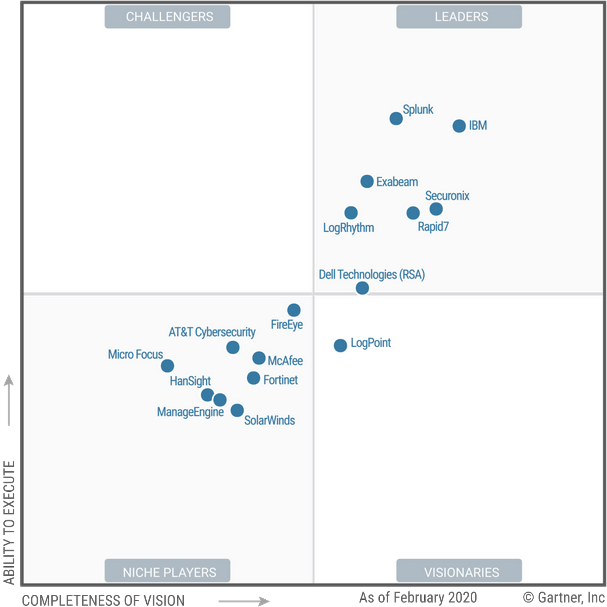
\includegraphics[width=10cm]{magic_quadro}}
\caption{Магический квадрат\cite{gartner2}}
\label{fig:magic_quad}
\end{figure}

Рассмотрим возможности анализа поведения пользователя продуктов лидеров IBM и Splunk.

\textbf{\textit{IBM QRadar SIEM}}

IBM QRadar SIEM - комплексное решение, вокруг которого построена платформа QRadar Security Intelligence Platform, включающая в себя множество компонентов. IBM QRadar User Behavior Analytics (UBA)\cite{ibm_uba} --- дополнительный модуль в рамках данной платфомы. IBM QRadar UBA использует готоые правила и модели машинного обучения для анализа пользовательского контекста\cite{ibm_uba} . В техническом отчете\cite{ibm_tech} говорится об использовании лишь контекста пользователей и упоминаются использование контента. Также, говорится об использовании ``множества'' методов машинного обучения, но не раскрывается, какие именно. Использование нейронных сетей не упоминется, а значит, скорее всего они не используются. Среди интересных особенностей можно выделить:
\begin{itemize}
\item Возможность, как поверхностного анализа всех пользователей, так и глубокое наблюдение за отдельными подозрительными пользователями
\item Создание и сравнение пользователей в разных списках наблюдения
\item Полная интеграция с системой IBM QRadar SIEM
\item Аггрегация данных журналов брандмауэра, информации о пользовании облачными приложеними, сетевых потоках и прочее.
\end{itemize}

\textbf{\textit{Splunk UBA}}

Компания Splunk имеет самостоятельный продукт Splunk UBA для анализа поведения пользователей. В white paper \cite{splunk_tech} подход Splunk UBA четырехэтапный:
\begin{enumerate}
\item Сбор данных. Платформа Splunk ---The Data-to-Everything Platform позволяет собирать огромное множество данных, включая такие данные как записи звонков, положение GPS и пр. О сборе контентных данных ничего не говорится.
\item Поиск аномалий. На этом шаге собираются аномальные факты поведения пользователей. Splunk используют обучение без учителя для детектирования аномалий(не уточняется, какие), причем модель обучается для каждого пользователя своя.
\item Аггрегация. На этом шаге анализируются большие объемы аномалий, найденных на втором шаге. Для этого используются предобученные алгоритмы машинного обучения без учителя (не уточняется, какие)
\item Исследование. Полученные результаты предоставляются аналитику в человекочитаемом виде для подробного анализа.
\end{enumerate}

Из обзора коммерческих продуктов видно, что на данных момент даже лидеры рынка UEBA-систем не анализируют контент пользователей, а также используют только классические методы машиннного обучения для обнаружения аномалий. Контент пользователей представляется огромным массивом данных, который мог бы быть учтен при анализе поведения пользователя, а более современных подходы в машинном обучении могли бы улучшить качество определения угроз. Таким образом, исследование и разработка современных методов машииного обучения для обнаружения внутренних угроз, использующих как контекстных поведенческих данных, так и контентных, является актуальной задачей.

\clearpage